\section{Know Thyself}

\begin{quote}
{\em Know thyself.} --- inscribed on the Temple of Apollo at Delphi
\end{quote}

Newell's advice cannot be followed until the strengths are named, and
self-report names them badly.
Hence, before diving deep into any literature, we first reverse
engineer the team from the record of its own papers.

Our instrument is the repertory grid of Kelly's personal construct
theory~\cite{kelly55}.
Kelly held that people make sense of a domain through bipolar
distinctions ({\em constructs}) of their own devising.
A grid is elicited by triads: pick three team members, ask which one
stands apart from the other two and on what dimension; each answer
yields one construct; repeat until no new dimensions appear; then rate
everyone on every construct.

Data collection took minutes.
For six of this paper's authors, an LLM agent fetched each author's
five most-cited papers of all time and of the last five years
(scanning some 1,200 paper records), coded them against the ICSE'27
research-track areas, then played triad interviewee.
Constructs agreeing above 90\% were merged.
Figure~\ref{fig:focus} shows the result after FOCUS sorting: rows and
columns reordered so similar neighbors adjoin, poles reversed to
align, and trees built by merging adjacent clusters
only.\footnote{Caveats: one rater (the agent), citation counts as the
sole proxy for strength, and two early-career authors rated on very
few papers.}

\begin{figure}[t]
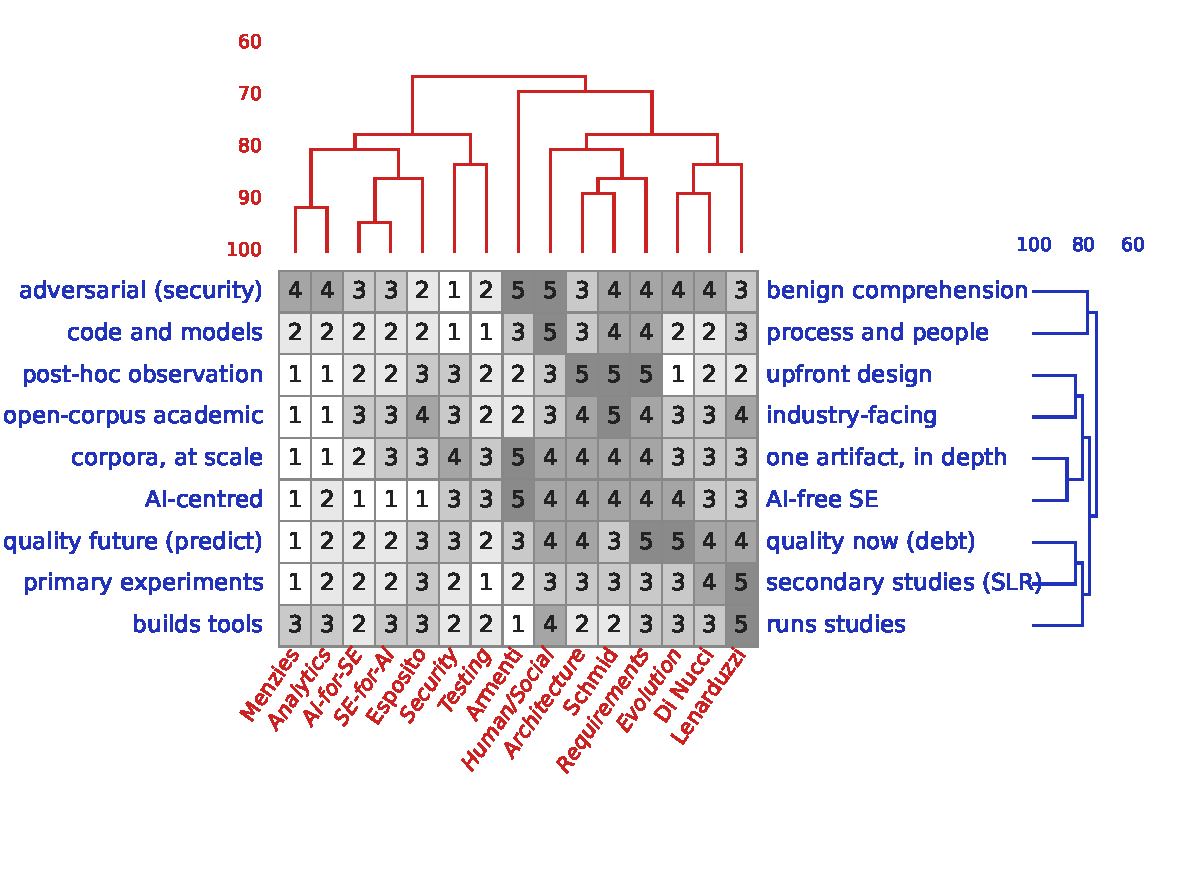
\includegraphics[width=\linewidth]{fig/focus_grid}
\caption{Repertory grid of six authors (upright columns)
plus the nine ICSE'27 areas as reference elements (italic columns; see
\S\ref{sec:map}).
Grey cells score each column from the left pole (1) to the right pole
(5) of each construct; trees join neighbors by percentage match;
regenerate via {\em make focus}.}
\label{fig:focus}
\end{figure}

The grid rewards three readings.
Firstly, near-synonyms: construct rows that merge early name one local
dimension twice.
In this team, working at corpus scale co-travels with being
AI-centred, as does primary experimentation with future-facing
prediction.
Secondly, birds of a feather: Lenarduzzi and Di Nucci match at around
90\%, a tight quality-and-evolution core that anchors the team.
Thirdly, complements: Schmid and Armenti lie farthest from that core,
so upfront design and single-artifact comprehension are scarce skills
here, present in exactly one member each.
Hence the grid is at once a division of labor and a price list of the
team's blind spots, computed before reading a single outside paper.
